\chapter{Bevezetés}
\label{chapIntroduction}

A szoftverfejlesztés a mai világunk egyik alapköve. 
Az informatika világa és a mi hétköznapijaink sem lennének képesek fejlődni a szorgos programozók munkája nélkül. 
Azonban a szoftver fejlesztés nem egy egyszerű dolog, főleg ha egy komplex programozási feladatra van szükség. 
Ilyenkor szinte biztosan nem egy ember fogja elkészíteni ezeket a programokat, így a munka érdemi része kevesebb feladatot ró a fejlesztőre viszont számos egyéb feladattal kell szembe néznie.
Ez a téma az informatika nem annyira szembetűnő oldaláról mutatja be. 
A mai világban gyakran hajlamosak vagyunk megfeledkezni arról, hogy az a kép amit elkattintunk a telefonunkkal hogyan is kerül fel a felhőbe és onnan a asztali számítógépünkre vagy akár a barátainkhoz valamilyen közösségi média platform használatának segítségével.
Nem egy program megszületését dokumentáltam hanem sokkal inkább azt, hogy egy komplex programhoz milyen háttér eszközök kellenek hogy elkészüljön.

Ezek a feladatok (ha jól elő vannak készítve) nagyon könnyen vehető akadályok. 
A csapatban való munka fontos részét alkotja a modern szoftverfejlesztésnek.
Ha egy mai informatikai céget meglátogatunk, azt láthatjuk hogy a programozók nem elszeparáltan hanem egy közös térben dolgoznak.
Például egyre népszerűbb a scrum módszer bevezetése az irodákban és minden reggel ennek megfelelően egy közös megbeszéléssel kezdőik.

A csapatmunkát komoly támogatási háttérrel szükséges ellátni. 
Gondok itt arra, hogy lehetőséget kell adni minden fejlesztő számára, hogy a fejlesztés állapotát nyomon tudják követni és a mások munkáját is könnyen feltudják használni vagy esetenként módosítani tudják azt. 
Ezeket a lehetőségeket nem egy egyszerű feladat megteremteni legyen szó tíz vagy akár százfős irodáról.

Persze ezen felül ha többen dolgoznak egy kódon akkor a csapatmunka gördülékenységét segíti elő bizonyos szabályok lefektetése.
Az ugyan olyan formátumú kód használata elengedhetetlen komplex programok megírásakor.

A programozókra komoly munka és rengeteg egyeztetés várna, ha nem léteznének úgynevezett verzió követő rendszerek.
Nem is lehetne olyan szoftver gyártó céget mondani mely nem használná valamely formában a Git-et.

Mindezeken felül még persze ott a dokumentáció is, hogy a kód később is vagy egy új kolléga számára is egyértelmű legyen.

“A Continuous Integration – azaz a folyamatos integráció

maga a CI fontossága
\pagebreak
\section{Motiváció}

Mostanra az informatikusnak tanulók között is sokkal izgalmasabb egy mobilfejlesztés vagy egy webfejlesztés.
Az látszik az van előtérben, végül is az ő munkájuk az ami igazán eljut a végfelhasználókhoz.
Ez teljesen megérthető hiszen a színes izgő-mozgó képek tengerével hogyan is vehetné fel a versenyt egy még a Mátrix c. kultuszfilmben is csak keveset látott terminál ablak fekete-zöld karakteri.
Pedig ez a világ az ami lehetővé teszi az eszközök közötti összeköttetést és a csillogó képekkel teli megjelenést.
Az ember azt gondolná hogy a programozók pontosan ismerik ezt a világot, pedig vannak akik ennél is mélyebbre mennek.
Ezek az emberek a rendszerüzemeltetők és az ők titkolt és rejtett világuk.
Pontosan ez tetszett meg nekem és ezért is szeretnék hasonló témában elkészíteni a feladatom.


%Azt ahogy már a bevezetésben megírtam a személyes motivációm egy része az az, hogy az üzemeltetés rejtélyes világát megismerhessem és eltanulhassam.
Természetesen ez talán még nem elég ahhoz hogy egy ilyen témába mélyen beleássa  magát az ember.
Már régebben is az foglalkoztatott hogy bizonyos játékoknak hogyan tudnék saját szervert csinálni hogy a barátainkkal igazán szabadon élvezhessük a játékok adta élményeket.

Szerencsére nekem az egyetem is lehetőséget adott ahhoz hogy ezzel a témával mélyebben is tudjak foglalkozni.
Dr. Tóth Zsolt konzulensem ajánlotta fel azt hogy ebben segítséget ad és természetesen egy célt is melyről komplexet és később majd a szakdolgozatomat is megírhatom.


\pagebreak
\section{Célkitűzés}
\paragraph{}
A célom azt volt, hogy a Miskolci Egyetem Általános Informatika Tanszékén az ILONA rendszeren dolgozó fejlesztőknek a munkáját segítsem. 
A fejlesztők jelenleg az építést és a tesztelést is manuálisan valósítják meg, ahogy ez a \ref{fig:jelenallapot} ábrán is látható. Ez a feladatom kiinduló állapota. 

\begin{figure}[h]
	\centering
	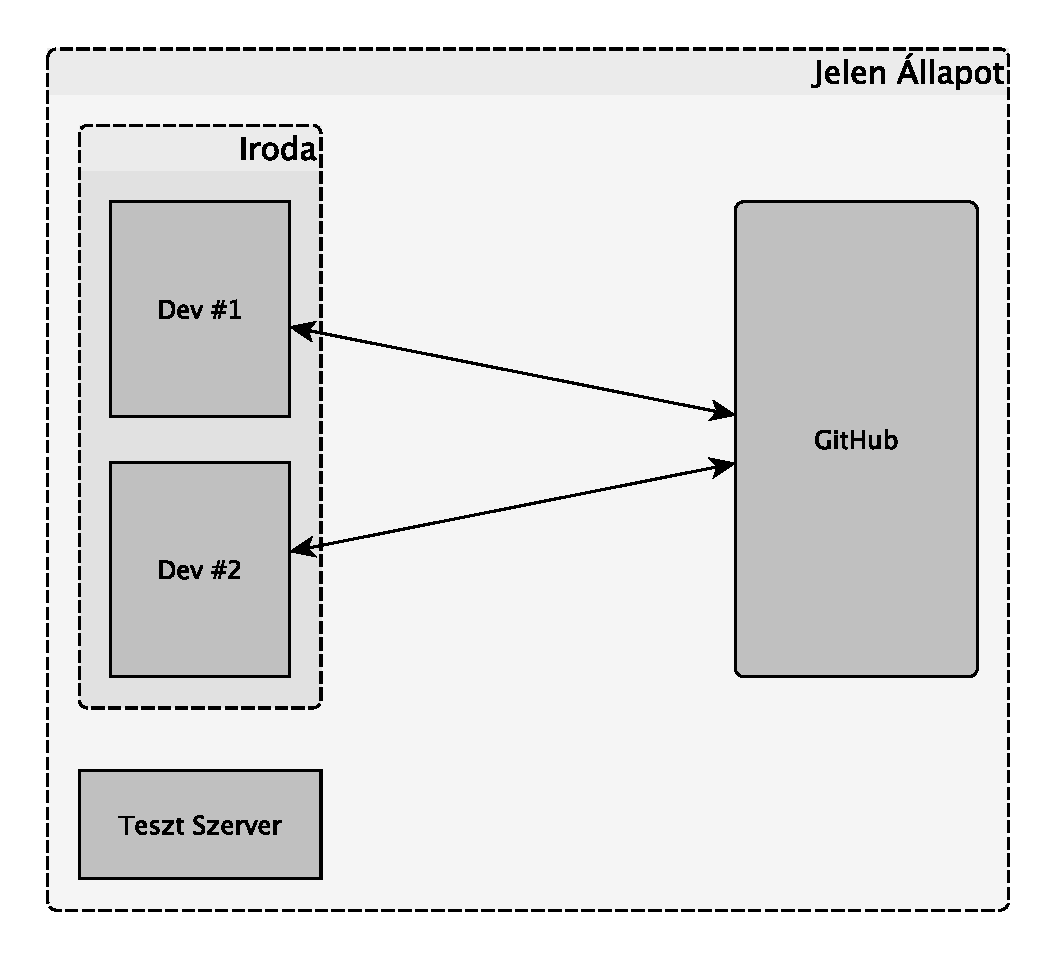
\includegraphics[width=0.7\linewidth]{figures/jelenallapot}
	\caption{Jelen Állapot}
	\label{fig:jelenallapot}
\end{figure}

Az új rendszernek a jelenlegi állapotnak több sajátosságát meg szerettem volna tartani és ezeken felül a már meglévő szerverekkel megvalósítani a rendszer működését. 
Fontosnak tartottam hogy a fejlesztők kizárólag a feladataik csökkenésével szembesüljenek és ne keljen új programokat, folyamatokat megtanulniuk. 
Kvázi ne látszódjon a háttérbe folyó változás és a jelenlegi rendszer szolgáltatás kiesésével se járjon az új rendszer bevezetése. 
Mivel az ILONA fejlesztése teljesen önerőből, támogatás nélkül valósul meg, ezért törekedtem arra hogy csak ingyenes, "opensource" alkalmazásokat használjak a feladathoz. 
--------------
A jelenlegi rendszer alapja az egyik legnépszerűbb ingyenes internetes verziókövető rendszer a GitHub. 
A GitHub-ot feltétlen meg akartam tartani az új rendszerben mivel egy elterjedten használt és kedvelt környezetnek tartom és ami még mellette szól az az ingyenessége. 
Ez a teszt szerver Maven segítségével építi és teszteli a megírt kódokat, ezért a következő amit a meglévő rendszerből át akartam vinni az újba az a Maven. 
A jelenlegi rendszer nem hatékony a munkavégzés során, mivel számos munkaidőt emészt fel a folyamat amely nem a fejlesztéssel kapcsolatos. 
--------------
\pagebreak
\paragraph{}
A fejlesztőknek az új rendszerben lényegében csak a GitHubbal és a kész JAR fájlokat tartalmazó repository szerverrel kell dolgozniuk a többi folyamatot automatikusan látná el a rendszer. 
A cél tehát egy olyan Automatikus Tesztelési Környezet megvalósítása, amely képes a GitHubról letölteni a kódokat akkor ha a kódban változás történik. 
Ezen felűl ha a tesztek és a buildelési folyamat is sikeresen végbement az elkészült fájlokat könnyen és szervezetten elérhetővé tennie egy repository szerveren. 
Ez a tervezett folyamat látható a \ref{fig:jovoallapot} ábrán. 


\begin{figure}[h]
	\centering
	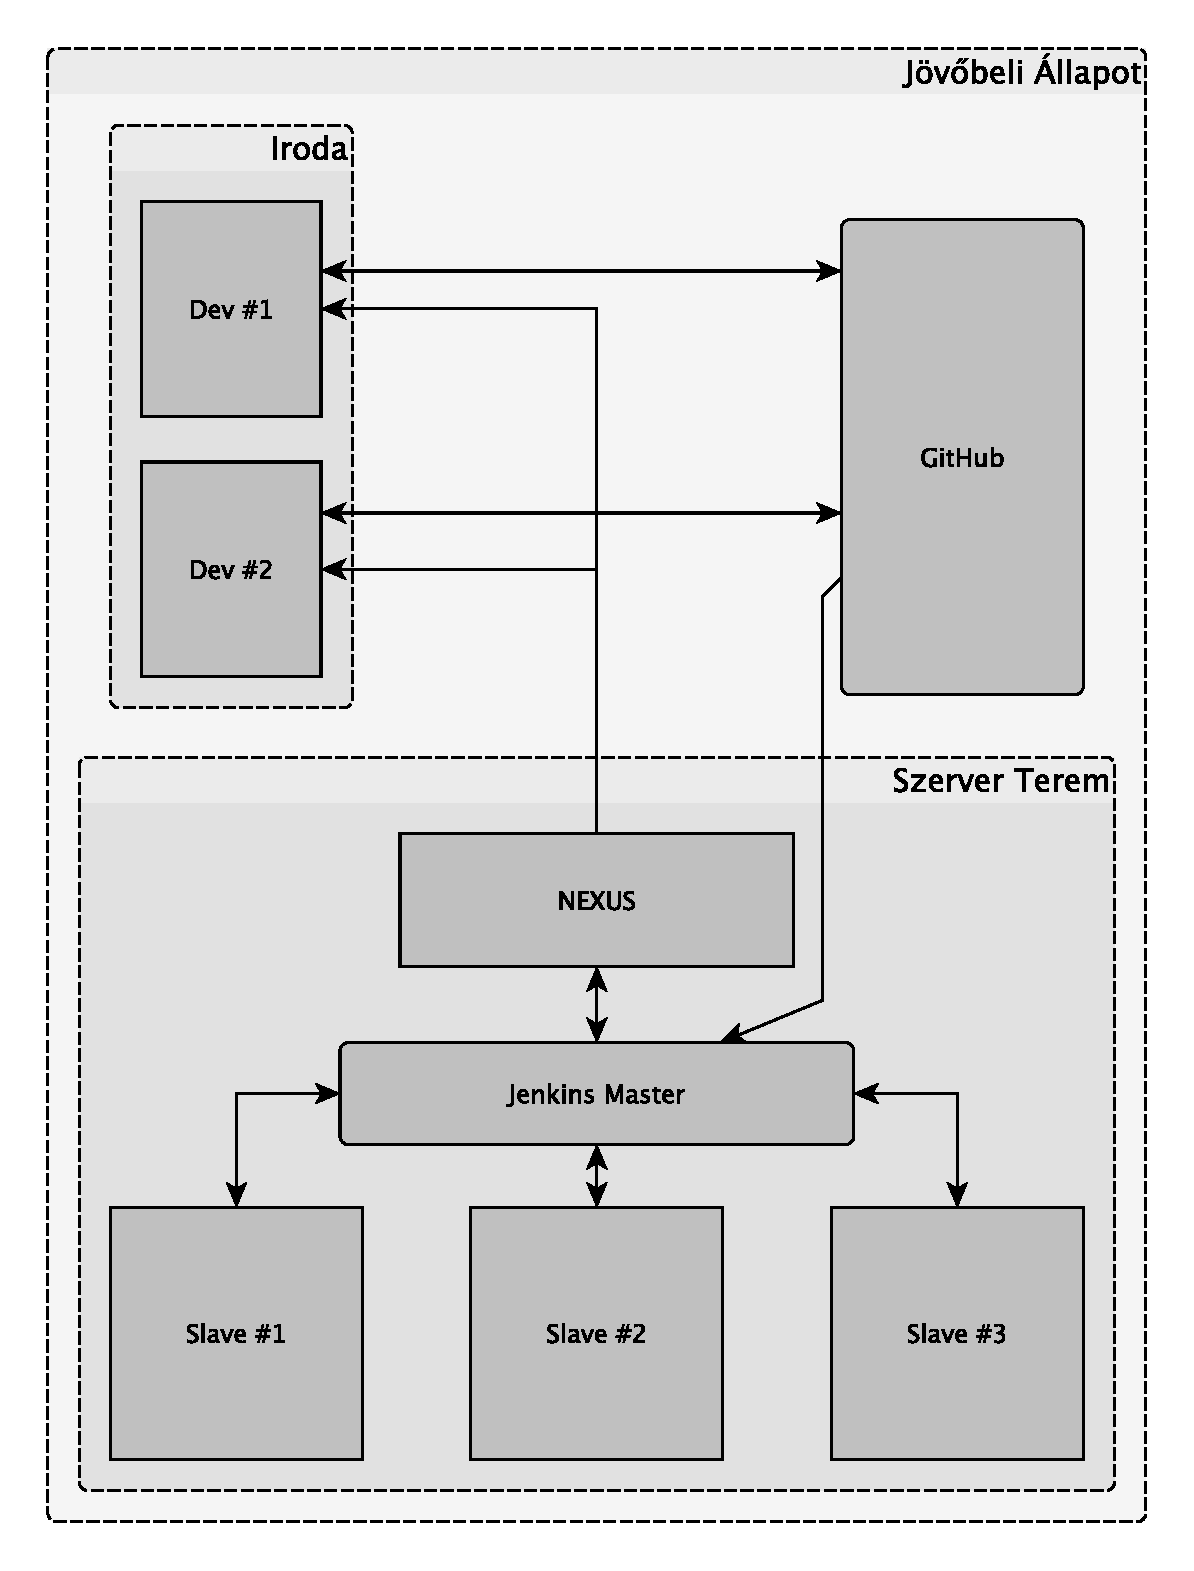
\includegraphics[width=0.7\linewidth]{figures/jovoallapot}
	\caption{Jövő Állapot}
	\label{fig:jovoallapot}
\end{figure}
